\section{Príklad č.~4} 

\subsection{Zadanie}
V obvode na obrázku nižšie v čase $t=\SI{0}{\second}$ zopne spinač S. Zostavte diferenciálnu rovnicu popisujúcu správanie obvodu na obrázku, ďalej ju upravte dosadením hodnôt parametrov. Vypočítajte analytické riešienie $i_L=f(t)$. Spravte kontrolu výpočtu dosadením do zostavenej diferenciálnej rovnice. \\

\begin{center}
\begin{minipage}{0.5\textwidth}
	\centering
	\begin{tabular}{|c|c|c|c|c|}
		\hline
		sk. & $U~[V]$&$L~[H]$ & $R~[\Omega]$ & $i_{L}(0)~[A]$ \\
		\hline
		B&30&10&20&15  \\
		\hline
	\end{tabular}
\end{minipage}
\end{center}

\begin{figure}[!h]
\centering
\begin{circuitikz}
\draw
(0,0) -- (3,0)
(0,2.5) to[dcvsource, v_=$U$] (0,0)
(0,2.5) to[nos, l=$S$] (0,5)
(0,5) to[R, l=$R_1$, v=$u_R$](3,5)
(3,5) to[L, l=$L$, v=$u_L$, i>_=$i_L$](3,0)
;
\end{circuitikz}
\caption{Pôvodný obvod}
\end{figure}

\subsection{Riešenie}
\textit{Po zopnutí spínača bude podľa II.KZ. platiť:}

\begin{equation*}
\begin{aligned}
-U+u_R+u_L=0
\end{aligned}
\end{equation*}

\textit{Vieme že:}
\begin{equation*}
\begin{aligned}
u_L=&L\frac{di}{dt} \\
u_R=&Ri
\end{aligned}
\end{equation*}

\textit{Vyjadrenie $u_R$ a $u_L$ z Ohmovho zákona:}

\begin{equation*}
\begin{aligned}
-U+Ri+L\frac{di}{dt}&=0 \\
Ri+L\frac{di}{dt}&=U
\end{aligned}
\end{equation*}

\textit{Vytvoríme charakteristickú rovnicu:}

\begin{equation*}
\begin{aligned}
L\lambda+R=0 \\
\lambda=-\frac{R}{L}=-\frac{1}{\tau}
\end{aligned}
\end{equation*}

\textit{Očakávame riešenie v tvare:}

\begin{equation*}
\begin{aligned}
i(t) = Ke^{\lambda t}+i_L
\end{aligned}
\end{equation*}
\clearpage
\textit{Výpočet:}

\begin{equation*}
\begin{aligned}
i_L =& \frac{U}{R} \; \; \;i_L(0) = \SI{15}{\ampere}\; \; \;t=0 \\
i_L(t) =& Ke^{\lambda*0}+i_L\\
i_L(0)=&K+i_L \\
15=&K+i_L \\
K=&15-i_L=15-\frac{U}{R} \\
i_L(t)=&(15-\frac{U}{R})e^{-\frac{R}{L}t}+\frac{U}{R} \\
i_L(t)=&\frac{U}{R}(1-e^{-\frac{R}{L}t})+15e^{-\frac{R}{L}t}
\end{aligned}
\end{equation*}

\textit{V našom prípade teda dostávame rovnicu:}
\begin{equation*}
\begin{aligned}
i_L(t)&=\frac{30}{20}(1-e^{-\frac{20}{10}t})+15e^{-\frac{20}{10}t}
\end{aligned}
\end{equation*}

\textit{Tú vieme ešte zjednodušiť:}

\begin{equation*}
\begin{aligned}
i_L(t)&=e^{-2t}\times \frac{27}{2} + \frac{3}{2}
\end{aligned}
\end{equation*}




\subsection{Overenie}

\textit{Skontrolovanie výslednej rovnice dosadením hodnôt:}

\begin{equation*}
\begin{aligned}
i_L(0)=&\frac{30}{20}(1-e^{-\frac{20}{10}*0})+15e^{-\frac{20}{10}*0} \\
15 =& 15
\end{aligned}
\end{equation*}

\textit{Analytická rovnica bola správna. Pre ďalšie overenie som namodeloval obvod v Partsime a vybral arbitrárny čas $t=\SI{1.5}{\second}$:}

\begin{figure}[h!]
    \centering
    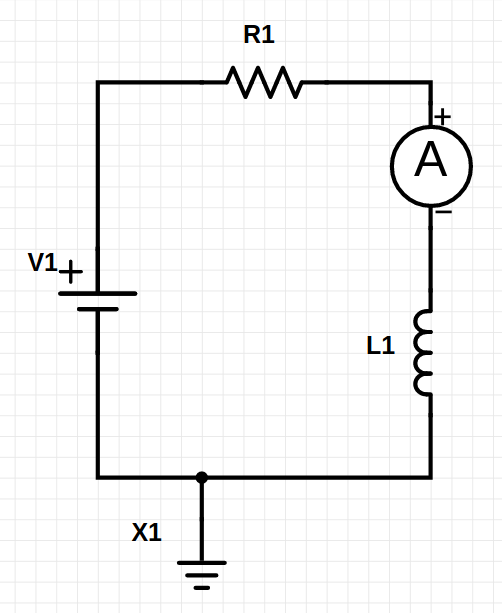
\includegraphics[width=0.3\textwidth]{img/partsim.png}
    \caption{Zapojenie obvodu v Partsim}
\end{figure}

Výpočet rovnicou ($t=\SI{1.5}{\second}$):

\begin{equation*}
\begin{aligned}
i_L(1.5)&=\frac{30}{20}(1-e^{-\frac{20}{10}*1.5})+15e^{-\frac{20}{10}*1.5} \\
i_L(1.5) &\approx \SI{2.172125423}{\ampere}
\end{aligned}
\end{equation*}

\newpage

Výsledok v Partsim:

\begin{figure}[h!]
    \centering
    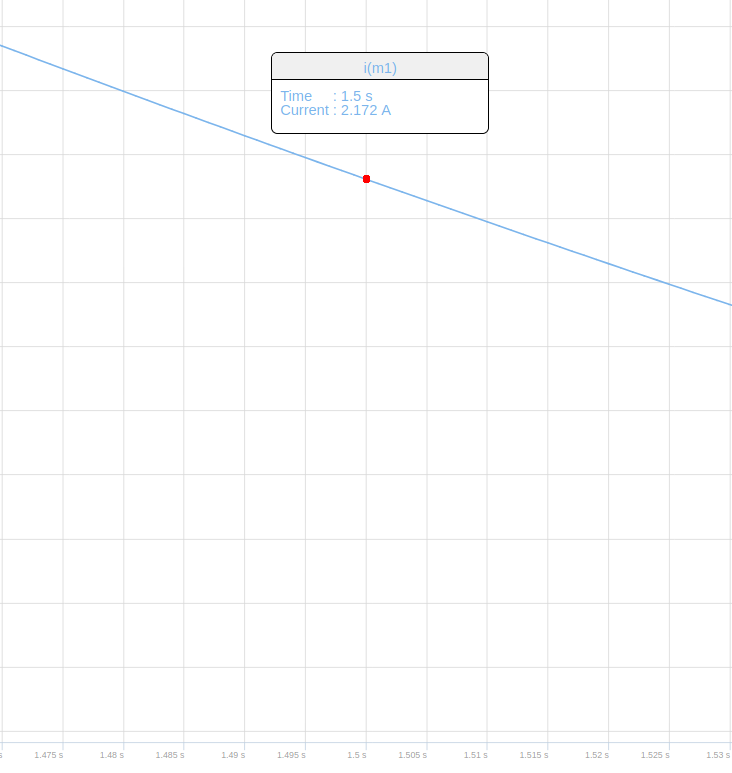
\includegraphics[width=0.8\textwidth]{img/graf.png}
    \caption{$i_L(\SI{1.5}{\second})$}
\end{figure}







